\documentclass{beamer}

% TODO: print out https://www.fuzzingbook.org/code/Intro_Testing.py

\usetheme{Boadilla}

%\includeonlyframes{current}

\usepackage{times}
\usefonttheme{structurebold}
\usepackage{listings}

\usepackage{pgf}
\usepackage{tikz}
\usepackage{alltt}
\usepackage[normalem]{ulem}
\usetikzlibrary{arrows}
\usetikzlibrary{automata}
\usetikzlibrary{shapes}
\usepackage{amsmath,amssymb}
\usepackage{rotating}
\usepackage{ulem}

\usetikzlibrary{arrows,automata,shapes}
\tikzstyle{block} = [rectangle, draw, fill=blue!20, 
    text width=5em, text centered, rounded corners, minimum height=2em]
\tikzstyle{bt} = [rectangle, draw, fill=blue!20, 
    text width=4em, text centered, rounded corners, minimum height=2em]

%\setbeamercovered{dynamic}
\setbeamertemplate{footline}[page number]{}
\setbeamertemplate{navigation symbols}{}
\usefonttheme{structurebold}

\title{Software Testing, Quality Assurance \& Maintenance---Lecture 3}
\author{Patrick Lam\\University of Waterloo}
\date{January 13, 2025}

\colorlet{redshaded}{red!25!bg}
\colorlet{shaded}{black!25!bg}
\colorlet{shadedshaded}{black!10!bg}
\colorlet{blackshaded}{black!40!bg}

\colorlet{darkred}{red!80!black}
\colorlet{darkblue}{blue!80!black}
\colorlet{darkgreen}{green!80!black}

\newcommand{\rot}[1]{\rotatebox{90}{\mbox{#1}}}
\newcommand{\gray}[1]{\mbox{#1}}

\newenvironment{changemargin}[1]{% 
  \begin{list}{}{% 
    \setlength{\topsep}{0pt}% 
    \setlength{\leftmargin}{#1}% 
    \setlength{\rightmargin}{1em}
    \setlength{\listparindent}{\parindent}% 
    \setlength{\itemindent}{\parindent}% 
    \setlength{\parsep}{\parskip}% 
  }% 
  \item[]}{\end{list}}



\begin{document}

\usebackgroundtemplate{\tikz\node[opacity=0.1]{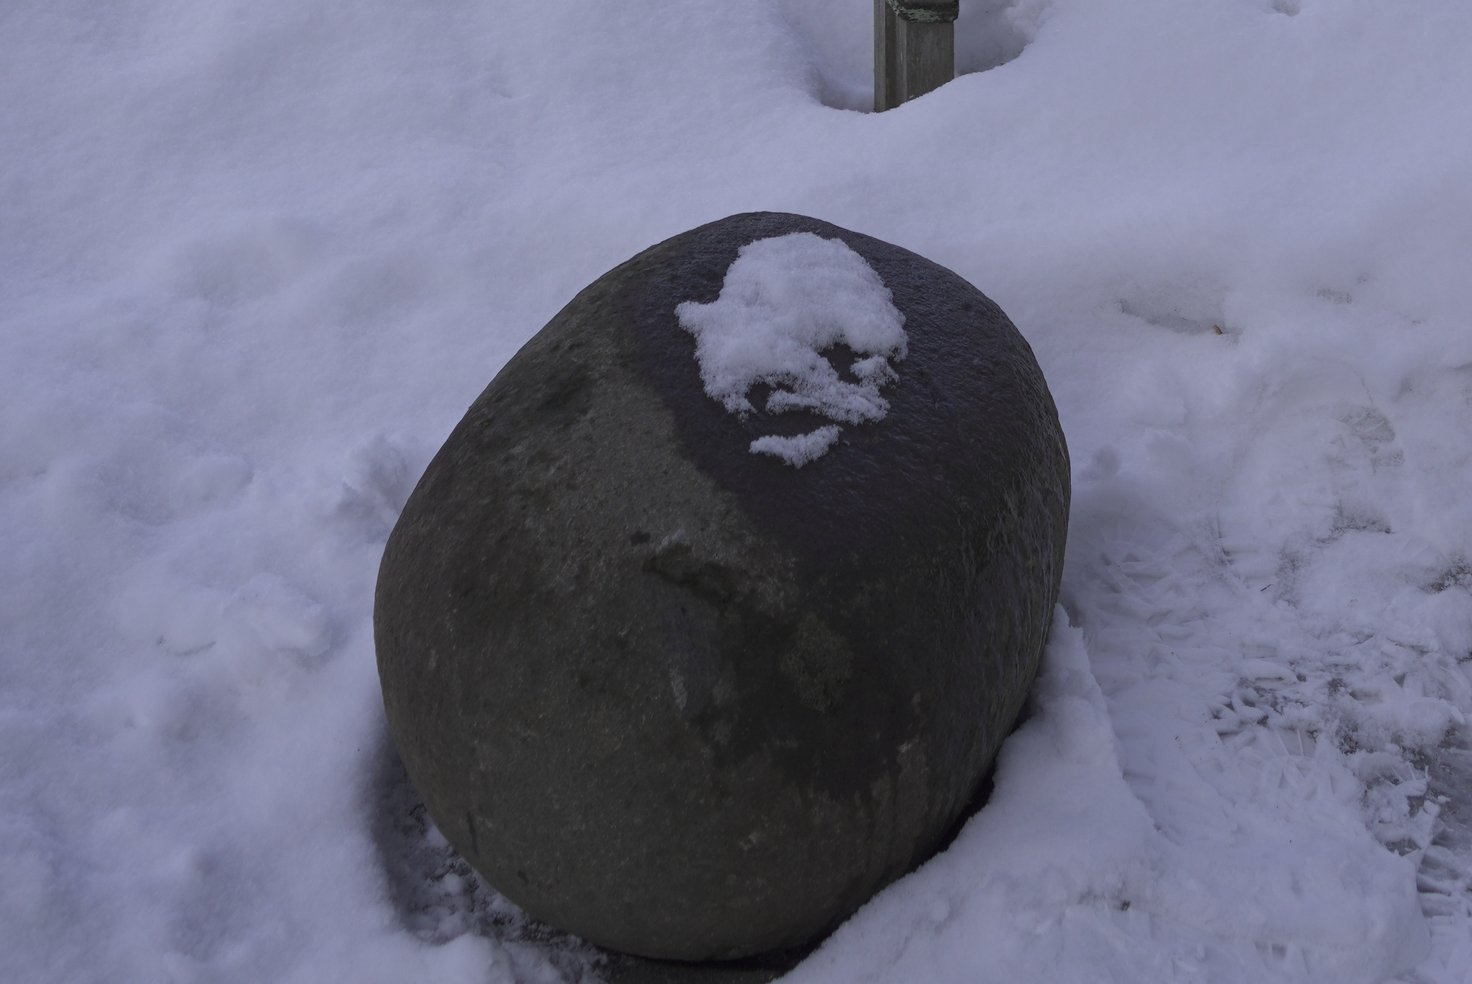
\includegraphics[width=\paperwidth]{L02/07172_about_banmochi_ishi_strength_and_grip_testing.JPG}};}
\begin{frame}
  \titlepage
\end{frame}

\begin{frame}
  \frametitle{Plan}

  \begin{changemargin}{2em}

    More on testing.\\[1em]

    Then, fuzzing.\\[2em]

    Later this week, shifting gears: \\
    \hspace*{2em} operational semantics!
  \end{changemargin}
\end{frame}

\part{When to stop? \\ Idea 1: Coverage}
\begin{frame}
  \partpage
\end{frame}

\begin{frame}
  \frametitle{How many tests?}
  \Large
  \begin{changemargin}{2em}
    Do you have enough test? How do you know?\\[1em]

    Test all inputs?\\[1em]

    State-of-the-industry: code coverage---\\[1em]
    \hspace*{2em} statement coverage, branch coverage.
  \end{changemargin}
\end{frame}

\usebackgroundtemplate{\tikz\node[opacity=0.1]{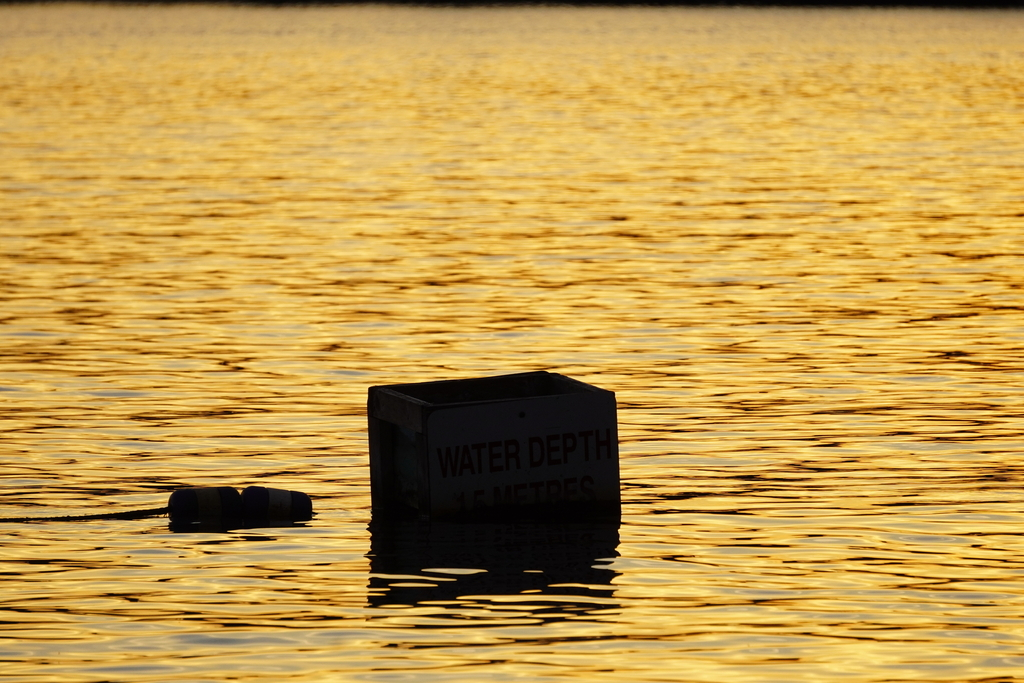
\includegraphics[width=\paperwidth]{L03/07882_box.JPG}};}
\begin{frame}
  \frametitle{Side note: white-box and black-box}
  \Large
  \hspace*{1em} When you write tests:\\[0.5em]
  \begin{changemargin}{2em}
    \alert{White-box testing:} you can look at the code;\\[1em]
    \alert{Black-box testing:} you can't look at the code.
  \end{changemargin}
\end{frame}

\usebackgroundtemplate{}
\begin{frame}
  \frametitle{Control-Flow Graphs}
  \large
  \begin{changemargin}{2em}
    Mostly people use lines of source code to evaluate coverage,
    but then your coverage depends on newlines.\\[1em]
    We are sometimes going to be more precise and use \alert{control-flow graphs}.
  \end{changemargin}
\end{frame}

\begin{frame}
  \frametitle{CFG nodes and edges}
  \large
  \begin{changemargin}{2em}
    Nodes: a node represents 0 or more statements;\\[1em]
    Edges: an edge $(s_1, s_2)$ indicates that $s_1$ may be followed by $s_2$ in an execution.
  \end{changemargin}
\end{frame}

\begin{frame}[fragile]
  \frametitle{Example: code for CFG}

  \Large
\begin{lstlisting}
  x = 5;
  for (z = 2; z < 17; z++)
    print(x);
\end{lstlisting}
  
\end{frame}

\begin{frame}[fragile]
  \frametitle{Reminder: how we compile}

  \begin{changemargin}{1em}
\begin{itemize}
\item lexing: \\
  \hspace*{1em} stream of characters $\rightarrow$ stream of tokens (if, while, strings)
\item parsing: \\
  \hspace*{1em} stream of tokens $\rightarrow$ concrete syntax tree
\item construction of Abstract Syntax Tree (AST): \\
  \hspace*{1em} cleans up the concrete syntax tree
\item conversion to Control Flow Graph: \\
  \hspace*{1em} AST $\rightarrow$ CFG
\item optimizations\\
  \hspace*{1em} CFG $\rightarrow$ CFG
\item convert to bytecode/machine code\\
  \hspace*{1em} CFG $\rightarrow$ bytecode/machine code
\end{itemize}
  \end{changemargin}
\end{frame}

\begin{frame}[fragile]
  \frametitle{Abstract Syntax Tree for Example}

  \begin{center}
\begin{tikzpicture}[->,>=stealth',shorten >=1pt,auto,node distance=1.5cm,
                    semithick,initial text=]

  \node[bt]           (1) {method()};
  \node[bt]           (2) [below left of=1] {x = 5};
  \node[bt]           (3) [below right of=1] {for};
  \node[bt]           (4) [right of=3,xshift=2em,yshift=-1em] {print(x)};
  \node[bt, text width=2.5em]           (5) [below left of=3,xshift=-3cm,yshift=-1em] {z = 2};
  \node[bt, text width=3.5em]           (6) [below of=3,xshift=-1.5cm] {z $<$ 17};
  \node[bt, text width=2.5em]           (7) [below right of=3,yshift=-1em] {z++};

  \path (1) edge node {} (2)
  (1) edge node {} (3)
  (3) edge node {body} (4)
  (3) edge node[left] {init} (5)
  (3) edge node[right] {term} (6)
  (3) edge node[right] {inc} (7);
\end{tikzpicture}
  \end{center}
\end{frame}


\begin{frame}[fragile]
  \frametitle{To a Control-Flow Graph}

  \begin{center}
\begin{tikzpicture}[->,>=stealth',shorten >=1pt,auto,node distance=1.5cm,
                    semithick,initial text=]

  \node[initial,bt]   (1)                     {1 (L1-2)};
  \node[bt]           (2) [below of=1]        {2 (L2)};
  \node[bt]           (3) [below of=2] {3 (L3)};
  \node[bt, text width=2em]           (4) [below left of=3,xshift=-1em,yshift=-1em] {4 (L4)};
  \node[bt, text width=2em]           (5) [below of=4,yshift=0em] {5 (L5)};
  \node[bt, text width=2em]           (6) [below of=5,yshift=0em] {6 (L6)};
  \node[bt, text width=2em]           (7) [below right of=3,xshift=1em,yshift=-1em] {7 (L7)};

  \path (1) edge node {} (2)
        (2) edge node {} (3)
        (3) edge node[left] {F} (4)
            edge [bend left] node {T} (7)
        (4) edge node {} (5)
        (5) edge node {} (6)
        (6.west) edge [bend left=45] node {} (3.west);
\end{tikzpicture}
  \end{center}
\end{frame}

\begin{frame}[fragile]
  \frametitle{Low-level Code}

\begin{changemargin}{2em}
\begin{lstlisting}
    x = 5
    z = 2
q0: if (z < 17) goto q1
    z = z + 1
    print (x)
    goto q0
q1: nop
\end{lstlisting}
\end{changemargin}
\end{frame}

\begin{frame}
  \frametitle{Basic Blocks}
\begin{changemargin}{2cm}
  Group together
  statements which always execute together (in sequential programs):
\end{changemargin}

\begin{center}
\begin{tikzpicture}[->,>=stealth',shorten >=1pt,auto,node distance=1.5cm,
                    semithick,initial text=]

  \node[initial,bt]   (1)                     {1 (L1-2)};
  \node[bt]           (2) [below of=1] {2 (L3)};
  \node[bt]           (3) [below left of=2,yshift=-1em] {3 (L4-6)};
  \node[bt]           (4) [below right of=3] {4 (L7)};

  \path (1) edge node {} (2)
        (2) edge node[left] {F} (3)
            edge [bend left] node {T} (4)
        (3) edge [bend left] node {} (2.west);
\end{tikzpicture}
\end{center}
\end{frame}

\begin{frame}
  \frametitle{Basic Block Definition}
  \begin{changemargin}{1cm}
    A \alert{basic block} is a sequence of instructions in the control-flow graph
    that has one entry point and one exit point.\\[1em]

    Usually want maximal basic blocks.\\[1em]

    May have multiple successors.\\[1em]

    No jumps into the middle of a basic block.
  \end{changemargin}
\end{frame}

\begin{frame}[fragile]
  \frametitle{Constructing Basic Blocks: if}
\begin{tabular}{ll|ll}
\begin{minipage}{.15\textwidth}
\scriptsize \begin{lstlisting}
if (z < 17)
  print (x);
else
  print (y);
\end{lstlisting}
\end{minipage} &
\begin{minipage}{.3\textwidth}
\begin{center}
\begin{tikzpicture}[->,>=stealth',shorten >=1pt,auto,node distance=1.5cm,
                    semithick,initial text=]

  \node[initial,bt]   (1)                     {1 (L1)};
  \node[bt,text width=2em]           (2) [below left of=1,yshift=-0.5em] {2 (L2)};
  \node[bt,text width=2em]           (3) [below right of=1,yshift=-0.5em] {3 (L4)};
  \node[bt]           (4) [below left of=3] {4};

  \path (1) edge node[left] {\tiny T} (2)
        (1) edge node[right] {\tiny F} (3)
        (2) edge node {} (4)
        (3) edge node {} (4);
\end{tikzpicture}
\end{center}
\end{minipage}&
\begin{minipage}{.25\textwidth}
\begin{center}
\begin{tikzpicture}[->,>=stealth',shorten >=1pt,auto,node distance=1.5cm,
                    semithick,initial text=]

  \node[initial,bt]   (1)                     {1 (L1)};
  \node[bt,text width=2em]           (2) [below left of=1,yshift=-0.5em] {2 (L2)};
  \node[bt]           (4) [below left of=3] {3};

  \path (1) edge node[left] {\tiny T} (2)
        (1) edge node[right] {\tiny F} (4)
        (2) edge node {} (4);
\end{tikzpicture}
\end{center}
\end{minipage}
& \scriptsize \begin{minipage}{.2\textwidth}
\begin{lstlisting}
if (z < 17)
  print(x);
\end{lstlisting}
\end{minipage}
\end{tabular}

~\\[1em]
Not talking about short-circuit evaluation.
\end{frame}

\begin{frame}[fragile]
  \frametitle{Constructing Basic Blocks: case/switch}

\begin{tabular}{ll}
\begin{minipage}{.45\textwidth}
\begin{lstlisting}
switch (n) {
  case `I': ...; break;
  case `J': ...; //fallthru
  case `K': ...; break;
}
// ...
\end{lstlisting}
\end{minipage} &
\begin{minipage}{.4\textwidth}
\begin{center}
\begin{tikzpicture}[->,>=stealth',shorten >=1pt,auto,node distance=1.5cm,
                    semithick,initial text=]

  \node[initial,bt]   (1)                     {1 (L1)};
  \node[bt, text width=3em]           (2) [below left of=1,xshift=-2em,yshift=-1em]  {2 (L2)};
  \node[bt, text width=3em]           (3) [below of=1]   {3 (L3)};
  \node[bt, text width=3em]           (4) [below right of=1,xshift=2em,yshift=-1em]   {4 (L4)};
  \node[bt, text width=3em]           (5) [below of=2]  {5 (L2')};
  \node[bt, text width=3em]           (6) [below of=3]  {6 (L3')};
  \node[bt, text width=3em]           (7) [below of=4]  {7 (L4')};
  \node[bt, text width=3em]           (8) [below of=6]  {8 (L6)};

  \path 
  (1) edge node[left,yshift=0.7em] {i} (2)
  (1) edge node {j} (3)
  (1) edge node {k} (4)
  (2) edge node {} (5)
  (3) edge node {} (6)
  (4) edge node {} (7)
  (6) edge node {} (7)
  (5) edge node {} (8)
  (7) edge node {} (8);
\end{tikzpicture}
\end{center}
\end{minipage}
\end{tabular}
\end{frame}

\begin{frame}[fragile]
  \frametitle{Constructing Basic Blocks: while}

\begin{tabular}{ll}
\begin{minipage}{.3\textwidth}
\begin{lstlisting}
x = 0; y = 20;
while (x < y) {
  x ++; y --;
}
\end{lstlisting}
\end{minipage} &
\begin{minipage}{.4\textwidth}
\begin{center}
\begin{tikzpicture}[->,>=stealth',shorten >=1pt,auto,node distance=1.5cm,
                    semithick,initial text=]

  \node[initial,bt]   (1)                     {1 (x = 0; y = 20)};
  \node[bt]           (2) [right of=1,xshift=2em]        {2 (L2)};
  \node[bt]           (3) [below right of=2,xshift=1em]  {3 (L3)};
  \node[bt]           (4) [below of=2,yshift=-2em]   {4};

  \path (1) edge node {} (2)
  (2) edge [bend left] node {$x < y$} (3)
  (3) edge [bend left] node {} (2)
  (2) edge node[left] {$\neg (x < y)$} (4);
\end{tikzpicture}
\end{center}
\end{minipage}
\end{tabular}
\end{frame}

\begin{frame}[fragile]
  \frametitle{Constructing Basic Blocks: for}

\begin{lstlisting}[basicstyle=\scriptsize \ttfamily]
for (Widget w : widgetList) {
  decorate(w);
}
\end{lstlisting}
  Either is OK:
\begin{tabular}{ll}
\begin{minipage}{.4\textwidth}
\begin{tikzpicture}[->,>=stealth',shorten >=1pt,auto,node distance=1.5cm,
                    semithick,initial text=]

  \node[initial,bt]   (1)                     {1 (L1)};
  \node[bt]           (3) [below right of=1,xshift=1em]  {2 (L2)};
  \node[bt]           (4) [below of=1,yshift=-2em]   {3 (L4)};

  \path 
  (1) edge [bend left] node {$w \in \mbox{\tt widgetList}$} (3)
  (3) edge [bend left] node {} (1)
  (1) edge node[left] {} (4);
\end{tikzpicture}
\end{minipage} &
\begin{minipage}{.5\textwidth}
\begin{tikzpicture}[->,>=stealth',shorten >=1pt,auto,node distance=1.5cm,
                    semithick,initial text=]

  \node[initial,bt,text width=8em]   (1)                     {it = wL.iterator()};
  \node[bt,text width=5.5em]            (2) [below of=1,yshift=.5em] {it.hasNext()};
  \node[bt,text width=7.5em]           (3) [below right of=2,xshift=2em,yshift=-.5em]  {w = it.next(); decorate(w);};
  \node[bt]           (4) [below of=2,yshift=-3em]   {3 (L4)};

  \path (1) edge node {} (2)
        (2) edge node[right] {\tiny T} (3)
        (3.north) edge [bend right] node {} (2.east)
        (2) edge node[left] {F} (4);
%  (1) edge [bend left] node {$w \in \mbox{\tt widgetList}$} (3)
%  (3) edge [bend left] node {} (1)
%  (1) edge node[left] {} (4);
\end{tikzpicture}
\end{minipage}
\end{tabular}
\end{frame}

\usebackgroundtemplate{\tikz\node[opacity=0.1]{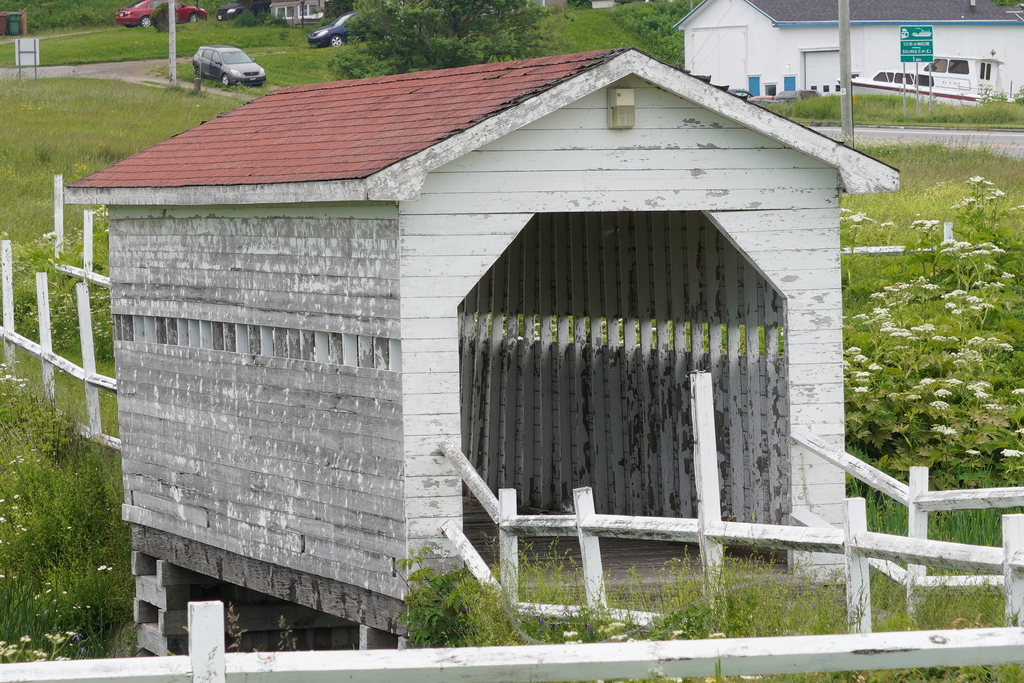
\includegraphics[width=\paperwidth]{L03/08467_covered_bridge.JPG}};}

\begin{frame}
  \frametitle{Back to Statement and Branch Coverage}

  \begin{changemargin}{2em}
    Given a test suite and a program,\\
    instrument the program to:
    \begin{itemize}
    \item count whether each statement (CFG node) is executed;
    \item count whether each branch (CFG edge) is taken.
    \end{itemize}
    ~\\
  
\alert{Statement coverage} is the fraction of statements (nodes) that are
executed by the test suite. \\[1em]
\alert{Branch coverage} is the fraction of branches (edges)
that are executed.
  \end{changemargin}
\end{frame}

\begin{frame}
  \frametitle{Example Code}
  \lstinputlisting{../code/l03/foo.py}
\end{frame}

\begin{frame}[fragile]
  \frametitle{Example Test Suite}
  \begin{lstlisting}
import unittest

from .foo import Foo

class CoverageTests(unittest.TestCase):
    def test_one(self):
        f = Foo()
        f.m(1, 2)

    def test_two(self):
        f = Foo()
        f.m(1, -2)

    def test_three(self):
        f = Foo()
        f.m(-1, 2)
  \end{lstlisting}
\end{frame}

\begin{frame}[fragile]
  \frametitle{Coverage Report}

  \begin{lstlisting}
Name             Stmts  Miss Branch BrPart Cover Missing
--------------------------------------------------------
l03/foo.py          11     2      8      2   79% 4, 11
l03/test_suite.py   12     0      0      0  100%
--------------------------------------------------------
TOTAL              124    98     46      2   21%
  \end{lstlisting}

\hspace*{2em}  HTML report also available.
  
\end{frame}

\begin{frame}
  \frametitle{On Coverage}
  \begin{changemargin}{2em}
    Can add missing test cases to visit all lines.\\[1em]

    Even with 100\% branch coverage, \\
    ~~one is missing an important behaviour: what if \texttt{b} is 0?
  \end{changemargin}
\end{frame}



\usebackgroundtemplate{}

\begin{frame}
  \frametitle{Infeasible Test Requirements}
  \begin{changemargin}{2em}
    Infeasible to reach 100\% coverage on real programs.

    How much is enough, and why is there a gap?
  \end{changemargin}
\end{frame}


\begin{frame}
  \frametitle{Some Real Coverage Data}
\begin{center}
  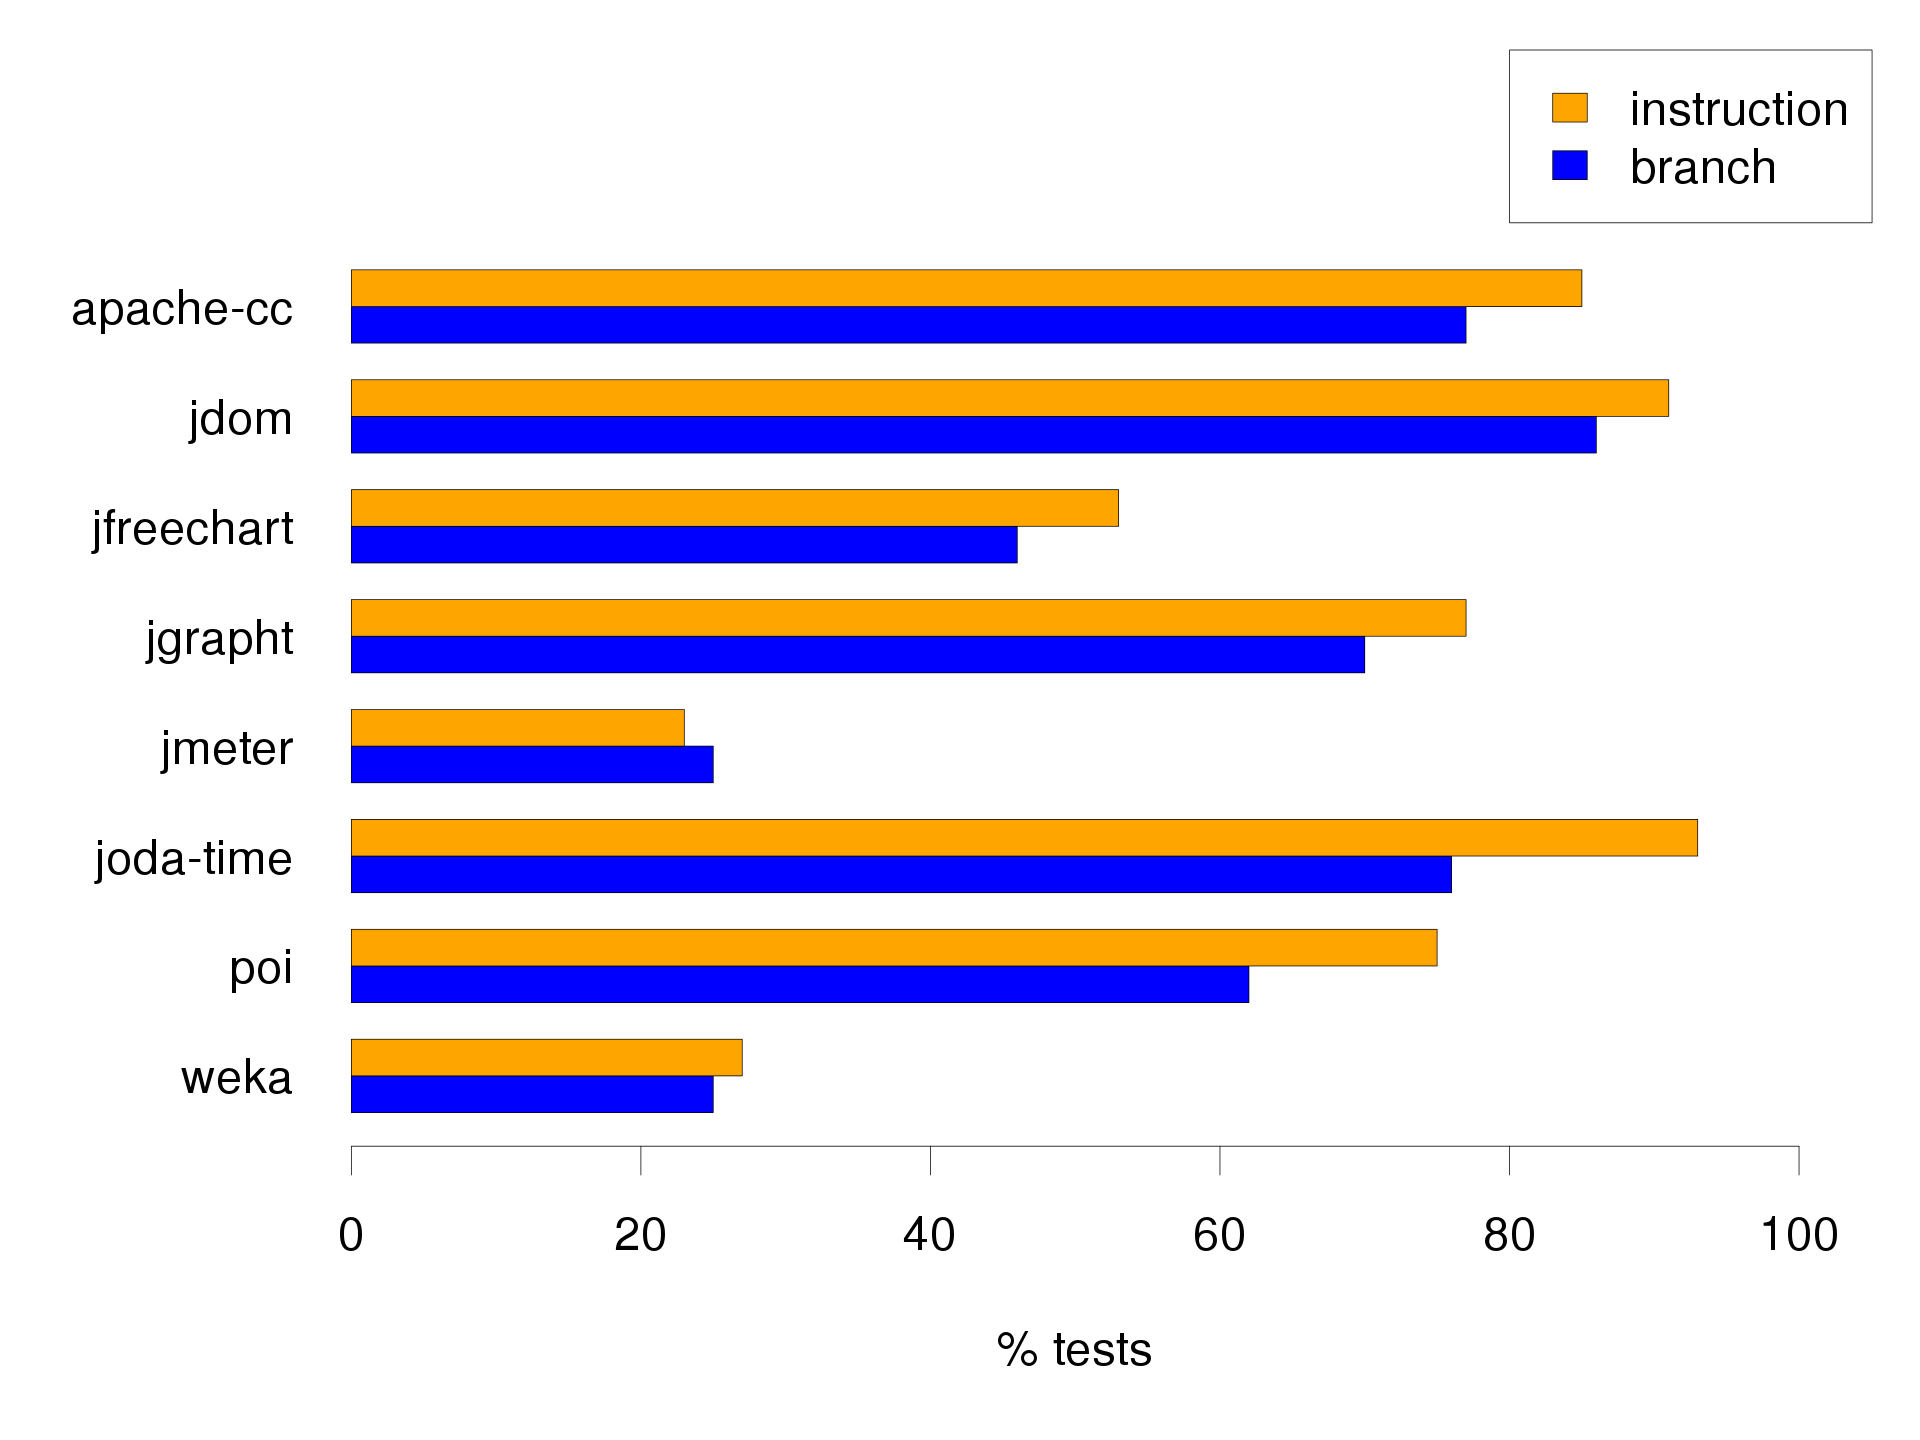
\includegraphics[height=3in]{L03/coverage.png}
\end{center}
\end{frame}

\begin{frame}
  \frametitle{Case Study: JUnit (4.11) the Artifact}
  \Large
\begin{center}
  \url{https://avandeursen.com/2012/12/21/line-coverage-lessons-from-junit/}
\end{center}
\end{frame}

\begin{frame}
  \frametitle{JUnit Measurements}
\begin{center}
  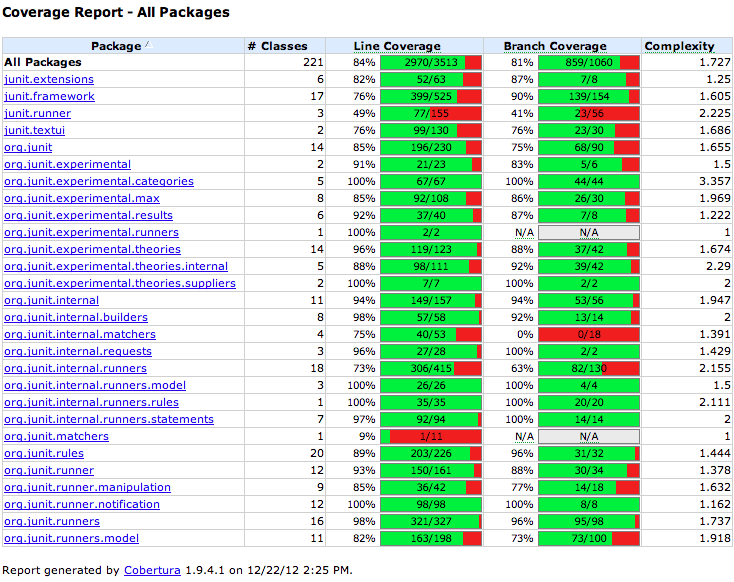
\includegraphics[height=3in]{L03/cobertura-junit.png}
\end{center}
\end{frame}

\begin{frame}
  \frametitle{JUnit Stats}
  \begin{changemargin}{2em}
    Overall instruction coverage: 85\%.\\[1em]
    13,000 lines of code, 15,000 lines of test.\\[1em]
    Consistent with industry average.
  \end{changemargin}
\end{frame}

\begin{frame}
  \frametitle{What's not covered? Deprecation}
  \begin{changemargin}{2em}
    \begin{itemize}
    \item deprecated code: 65\% instruction coverage
    \item nondeprecated code: 93\% instruction coverage
    \end{itemize}
    ~\\[1em]
    \begin{itemize}
    \item newer code (in {\tt org.junit.*}): 90\% instruction coverage
      \item older code (in {\tt junit.*}): 70\% instruction coverage
    \end{itemize}

    ~\\[1em]
  (Why is this? Perhaps the coverage decreased over time for the deprecated code, since
no one is really maintaining it anymore, and failing test cases just get removed.)
\end{changemargin}
\end{frame}

\begin{frame}
  \frametitle{A Whole Untested Class}

  \begin{changemargin}{2em}
    Blogpost author found one class that was completely untested!\\[1em]

    There were tests.\\
    But the tests never got run, because they were never added to CI.\\[1em]
    They also failed when run. (You don't run it, it doesn't work.)
  \end{changemargin}
\end{frame}

\begin{frame}[fragile]
  \frametitle{The Usual Suspects 1: Too Simple to Test}

  \begin{changemargin}{2em}
\begin{lstlisting}[language=Java]
  public static void assumeFalse(boolean b) {
    assumeTrue(!b);
  }
\end{lstlisting}

\begin{lstlisting}[language=Java]
  /**
  * Override to set up your specific external resource.
  *
  * @throws if setup fails (which will disable {@code after}
  */
  protected void before() throws Throwable {
    // do nothing
  }
\end{lstlisting}
  \end{changemargin}
\end{frame}

\begin{frame}[fragile]
  \frametitle{The Usual Suspects 2: Dead by Design}
  \begin{changemargin}{2em}
\begin{lstlisting}[language=Java]
  /**
  * Protect constructor since it is a static only class
  */
  protected Assert() { }
\end{lstlisting}

\begin{lstlisting}[language=Java]
  // should never be executed:
  catch (InitializationError e) {
    throw new RuntimeException(
    "Bug in saff's brain: " +
    "Suite constructor, called as above, should always complete");
  }
\end{lstlisting}

\begin{lstlisting}[language=Java]
  // unreachable
  try {
    ...
  } catch (InitializationError e) {
    return new ErrorReportingRunner(null, e); // uncovered
  }
\end{lstlisting}
  \end{changemargin}
\end{frame}

\begin{frame}
  \frametitle{Thoughts on JUnit Coverage}
\begin{changemargin}{2em}
  JUnit: written by people who care about testing.\\[1em]

  Non-deprecated code: 93\% instruction coverage, \\
  \hspace*{2em} i.e. $\le$ 2--3 untested lines of code per method.\\[1em]

  Probably OK to have lower coverage for deprecated code.\\[1em]

  Don't forget that what is in the tests matters too!
\end{changemargin}
\end{frame}

\part{Fuzzing}
\begin{frame}
  \partpage
\end{frame}

  \end{document}
